\documentclass[mingoth]{kut-paper}
\usepackage[dvipdfmx]{graphicx}
\usepackage{lmodern}
\usepackage{textcomp}
\usepackage{latexsym}
\usepackage{url}

\ScInfo
\Bachelor	%% 卒業研究論文梗概の場合
%\Project	%% プロジェクト研究報告書梗概の場合
%\Seminar	%% 特別研究セミナー課題研究報告書梗概の場合
%\Master	%% 修士学位論文(情報システム工学コース)梗概の場合
%\Doctorate	%% 博士学位論文(情報システム工学コース)梗概の場合
% \English	%% 英語の場合

%\figurespagefalse		%% 図目次を出力しない場合
%\tablespagefalse		%% 表目次を出力しない場合

\years{平成xx}
\title{Title}
\titlelength{20}		%% 表紙の表題の行長(全角文字数<20, default=19)
\Etitle{Title}
\idnumber{Your ID}
\author{Your Name}
\Eauthor{Your Name}
\advisor{Advisor}
\date{\today}
\abstract{}
\keyword{}
\Eabstract{}

\Ekeyword{}

\begin{document}
\maketitle

\chapter{概論}

本論文は,高知工科大学情報学群 \cite{kut} の論文テンプレートである.
\TeX ファイルの内容は,内容に応じて自由に変更して構わない.
ただし,\TeX ファイルからの参考文献の参照が一つもないと,
参考文献リストを BiBTeX で出力している関係から,うまくコンパイルできないので注意すること.
したがって,他の参考文献を追加した後 \verb|\cite{kut}| を消せば良い.

\begin{figure}[ht]
  \centering
  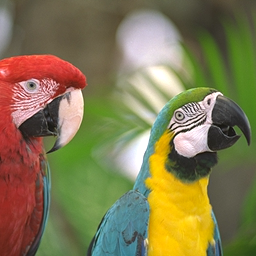
\includegraphics[width=8cm]{images/Parrots.bmp}
  \caption{サンプル画像}
  \label{fig:sample}
\end{figure}

% 参考文献リスト
\bibliography{refs}
\bibliographystyle{sieicej}

% 参考文献の文字間隔が広く空いて出力される場合は,以下を使う
%
% \begin{flushleft}
%   \bibliography{refs}
%   \bibliographystyle{sieicej}
% \end{flushleft}

\end{document}
